\section{Results}
\label{sec:results}
% Give the outcomes for each research question in the form of a table or graphic (with caption).
% Write about your results here. Good captions to tables and/or figures are key.

\subsection{Transformer models}

% Show loss curve of UNet, ViT and MVTS transformer. 
In this section, we show the results during the pretraining of the transformer models

We can conclude that the ViT does not extract any additional features from the data, since the loss plateus to the same value. However, due to extra trainable parameters the ViT is much slower. The mvts model is not a good model.

The pretrained ViT model was used for the evaluation of Peregrine. Round 2 training of ViT took 11 hours, so was terminated not to waste computing budget.

AUROC for 15 features after 24 hours of training.

Generally speaking, the ViT extracts the extrinsic parameters better than U-Net, while U-Net is better for the intrinsic parameters. This could be because the extrinsic parameters tend to affect the waveform on a more global level, while the intrinsic parameters affect the waveform more locally. Due to the self-attention of the transformer , it might be better at detecting the more global relationships.


\begin{table}
    \caption{Loss values for each of the parameters}
    \begin{tabular}{lrrr}
    \toprule
    Parameter & MTS & ViT & U-Net \\
    \midrule
    $q$ & -0.231 & -0.295 & -0.300 \\
    $M$ & -0.542 & -0.676 & -0.701 \\
    $\theta_{jn}$ & -0.327 & -0.463 & -0.426 \\
    $\phi_c$ & 0.000 & 0.000 & 0.000 \\
    $\theta_1$ & -0.107 & -0.167 & -0.174 \\
    $\theta_2$ & -0.018 & -0.036 & -0.036 \\
    $a_1$ & -0.078 & -0.104 & -0.132 \\
    $a_2$ & -0.005 & -0.008 & -0.007 \\
    $\phi_{12}$ & 0.000 & 0.000 & 0.000 \\
    $\phi_{jl}$ & -0.199 & -0.291 & -0.287 \\
    $d_L$ & -0.196 & -0.294 & -0.291 \\
    $\delta$ & -0.830 & -0.923 & -0.899 \\
    $\alpha$ & -1.020 & -1.085 & -1.066 \\
    $\psi$ & -0.063 & -0.117 & -0.090 \\
    $t_c$ & -0.965 & -1.104 & -1.105 \\
    \bottomrule
    \end{tabular}
\end{table}


\begin{figure}
  \centering
  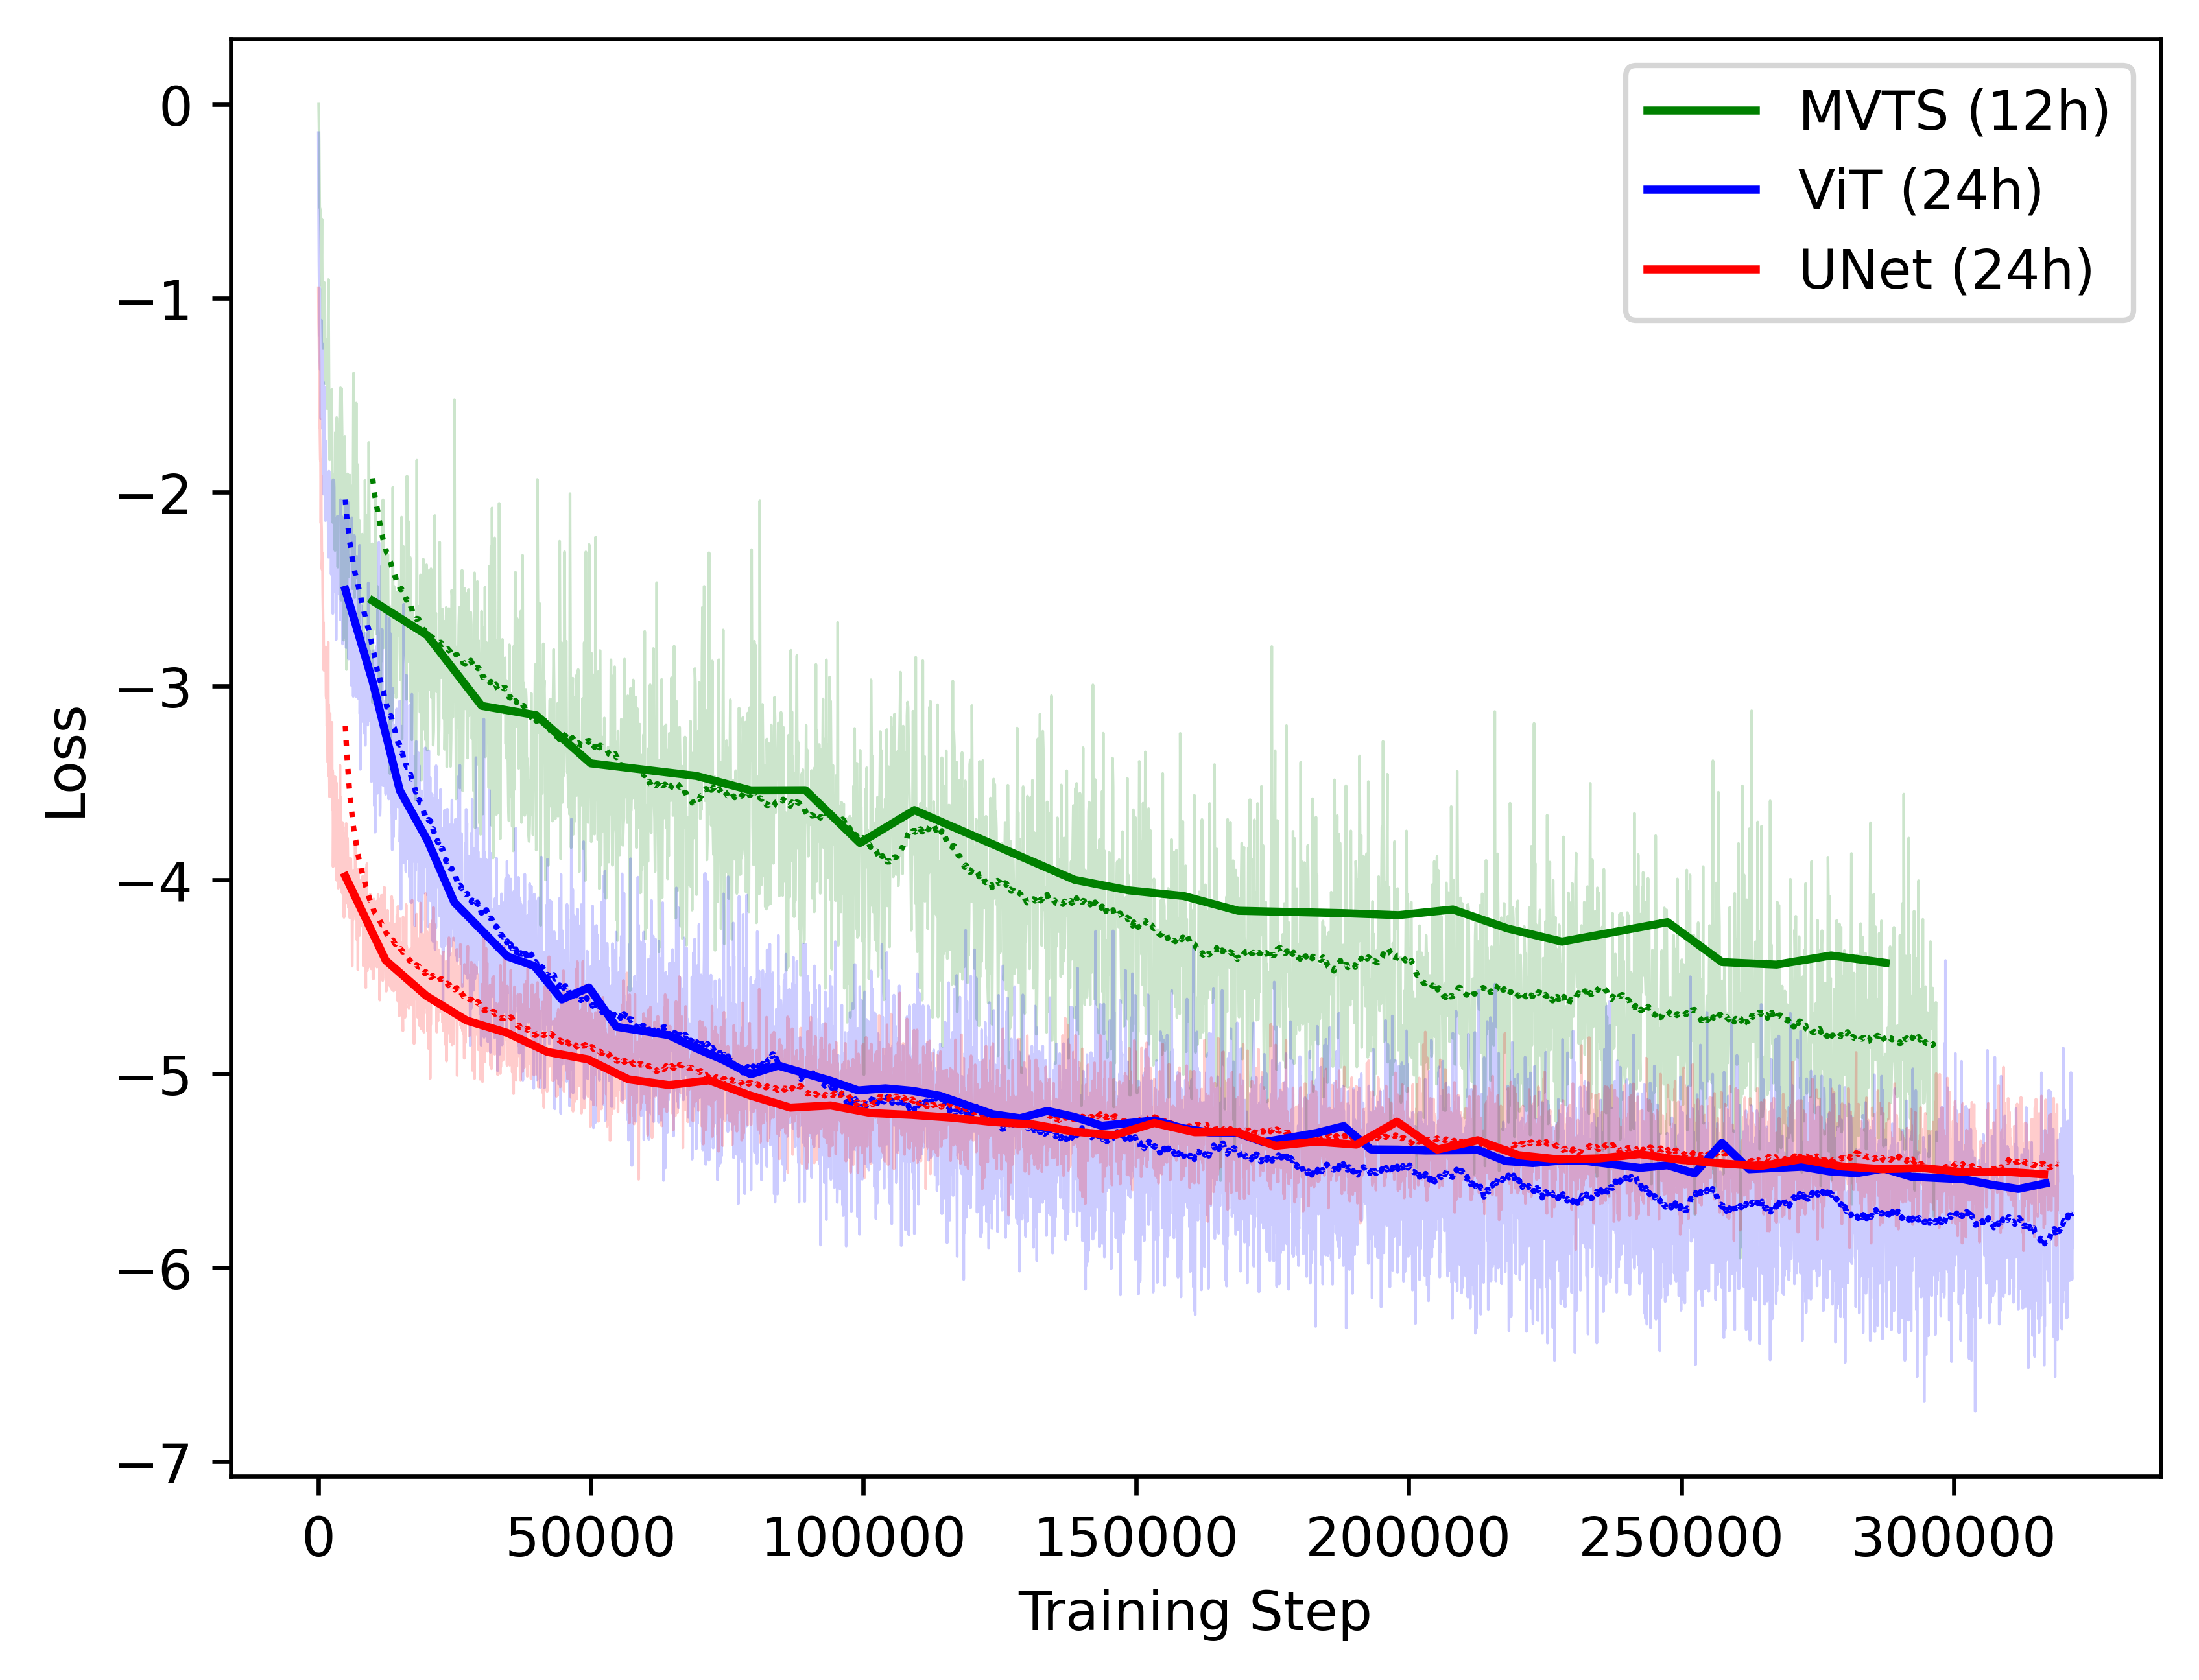
\includegraphics[width=1\linewidth]{media/images/Pretraining_loss_curve.png}
  \caption{Training curves for the two transformer models and U-Net. The original training loss is shown in transparent, the smoothed average (period 50) of the training loss is shown in dotted lines, and the validation loss is shown as a solid line.}
  \Description[<short description>]{<long description>}
  \label{fig:pretain_loss_curve}
\end{figure}

\subsection{Peregrine Network}



\begin{table}
\caption{Network performance of different network architectures for Peregrine}
\hspace{-2cm}
\begin{tabular}{lrrrrrrr}
\toprule
\multicolumn{1}{p{0.5cm}}{\raggedright Network}  & 
\multicolumn{1}{p{0.5cm}}{\raggedleft Round}  &
\multicolumn{1}{p{1cm}}{\raggedleft Num \\ Epochs} &
\multicolumn{1}{p{1cm}}{\raggedleft Num \\ Steps} &
\multicolumn{1}{p{1cm}}{\raggedleft Sampling \\ Fraction} &
\multicolumn{1}{p{0.75cm}}{\raggedleft Train \\ Loss} &
\multicolumn{1}{p{0.75cm}}{\raggedleft Test \\ Loss} &
\multicolumn{1}{p{1cm}}{\raggedleft Avg \\ AUROC} \\
\midrule
UNet & 1 & 104 & 10504 & 4.98e-03 & -4.71 & -4.22 & 0.706 \\
UNet & 2 & 79 & 16432 & 2.66e-05 & -4.78 & -4.65 & 0.738 \\
UNet & 3 & 77 & 23793 & 2.38e-06 & -4.71 & -4.47 & 0.741 \\
UNet & 4 & 74 & 30858 & 1.61e-06 & -4.14 & -4.43 & 0.741 \\
UNet & 5 & 90 & 37530 & 8.15e-07 & -4.43 & -4.39 & 0.742 \\
UNet & 6 & 60 & 31440 & 6.03e-07 & -4.19 & -4.25 & 0.736 \\
\midrule
Att UNet & 1 & 74 & 7474 & 1.04e-02 & -4.48 & -4.16 & 0.710 \\
Att UNet & 2 & 78 & 16224 & 2.21e-05 & -4.83 & -4.65 & 0.731 \\
Att UNet & 3 & 58 & 17922 & 5.59e-06 & -4.35 & -4.35 & 0.735 \\
Att UNet & 4 & 54 & 22518 & 2.76e-06 & -4.32 & -4.27 & 0.736 \\
Att UNet & 5 & 87 & 36279 & 2.51e-06 & -4.38 & -4.16 & 0.735 \\
Att UNet & 6 & 83 & 43492 & 1.74e-06 & -4.09 & -4.19 & 0.734 \\
\midrule
UNet 5\% & 1 & 68 & 6868 & 4.21e-03 & -5.03 & -4.43 & 0.716 \\
UNet 5\% & 2 & 65 & 13520 & 5.40e-05 & -4.85 & -4.49 & 0.731 \\
UNet 5\% & 3 & 75 & 23175 & 7.71e-06 & -4.05 & -4.33 & 0.736 \\
UNet 5\% & 4 & 48 & 20016 & 4.67e-06 & -4.09 & -4.41 & 0.743 \\
UNet 5\% & 5 & 60 & 25020 & 3.91e-06 & -4.27 & -4.46 & 0.743 \\
UNet 5\% & 6 & 30 & 15720 & 3.52e-06 & -4.74 & -4.38 & 0.741 \\
\midrule
UNet 10\% & 1 & 39 & 3939 & 4.31e-02 & -3.98 & -3.89 & 0.689 \\
UNet 10\% & 2 & 35 & 7280 & 3.72e-03 & -3.67 & -3.76 & 0.706 \\
UNet 10\% & 3 & 58 & 17922 & 4.33e-05 & -4.42 & -4.62 & 0.732 \\
UNet 10\% & 4 & 57 & 23769 & 1.14e-05 & -4.54 & -4.27 & 0.735 \\
UNet 10\% & 5 & 30 & 12510 & 8.17e-06 & -3.90 & -3.96 & 0.725 \\
UNet 10\% & 6 & 56 & 29344 & 4.87e-06 & -4.08 & -4.31 & 0.738 \\
\midrule
ViT & 1 & 30 & 12540 & 4.37e-05 & -6.15 & -5.58 & 0.753 \\
ViT & 2 & 60 & 50460 & 2.03e-06 & -5.82 & -5.28 & 0.757 \\
\bottomrule
\end{tabular}
\end{table}


Look at different parameters for round 6.
Compare the four different UNet models.
To compare the network performances we look at the number of epochs required per round, and the sampling fraction. We choose the sampling fraction because it is an indicator of how much the algorithm was able to truncate the priors, and is thus a proxy measurement of the precision capabilities of the network. Apart from the first round, we cannot easily compare loss functions 

Transformer very slow due to many trainable, even pretrained and retraining.

Pruned networks are faster to train, but lose precision as the rounds progress.

\begin{table}
\caption{Round 6 AUC and loss values}
\hspace*{-2cm}
\begin{tabular}{lrrrrrrrr}
\toprule
Param & 
\multicolumn{1}{p{0.3cm}}{\raggedright UNet}  & 
\multicolumn{1}{p{0.3cm}}{\raggedleft Att UNet}  &
\multicolumn{1}{p{0.3cm}}{\raggedleft UNet 10\%}  &
\multicolumn{1}{p{0.3cm}}{\raggedleft UNet 5\%}  &
\multicolumn{1}{p{0.3cm}}{\raggedright UNet}  & 
\multicolumn{1}{p{0.3cm}}{\raggedleft Att UNet}  &
\multicolumn{1}{p{0.3cm}}{\raggedleft UNet 10\%}  &
\multicolumn{1}{p{0.3cm}}{\raggedleft UNet 5\%}  \\
\midrule
$q$ & 0.765 & 0.756 & 0.744 & 0.761 & -0.282 & -0.257 & -0.246 & -0.275 \\
$M$ & 0.833 & 0.817 & 0.825 & 0.817 & -0.448 & -0.403 & -0.428 & -0.415 \\
$\theta_{jn}$ & 0.800 & 0.795 & 0.815 & 0.812 & -0.352 & -0.343 & -0.391 & -0.386 \\
$\phi_c$ & 0.499 & 0.500 & 0.501 & 0.506 & 0.000 & 0.000 & 0.000 & -0.000 \\
$\theta_1$ & 0.756 & 0.754 & 0.746 & 0.748 & -0.243 & -0.240 & -0.221 & -0.226 \\
$\theta_2$ & 0.638 & 0.640 & 0.627 & 0.628 & -0.069 & -0.069 & -0.055 & -0.058 \\
$a_1$ & 0.725 & 0.714 & 0.715 & 0.722 & -0.193 & -0.180 & -0.170 & -0.187 \\
$a_2$ & 0.573 & 0.571 & 0.567 & 0.579 & -0.022 & -0.023 & -0.019 & -0.023 \\
$\phi_{12}$ & 0.499 & 0.498 & 0.502 & 0.503 & 0.000 & 0.001 & 0.000 & -0.000 \\
$\phi_{jl}$ & 0.856 & 0.892 & 0.890 & 0.901 & -0.503 & -0.620 & -0.594 & -0.633 \\
$d_L$  & 0.828 & 0.812 & 0.814 & 0.818 & -0.444 & -0.400 & -0.394 & -0.411 \\
$\delta$  & 0.848 & 0.846 & 0.856 & 0.859 & -0.496 & -0.480 & -0.506 & -0.519 \\
$\alpha$  & 0.858 & 0.841 & 0.854 & 0.853 & -0.520 & -0.468 & -0.509 & -0.501 \\
$\psi$ & 0.714 & 0.715 & 0.741 & 0.746 & -0.175 & -0.177 & -0.217 & -0.231 \\
$t_c$ & 0.854 & 0.865 & 0.873 & 0.854 & -0.515 & -0.545 & -0.565 & -0.511 \\

\bottomrule
\end{tabular}
\end{table}

\subsection{Peregrine Run Strategy}

In this section we show the results of varying the number of simulations, and the different sampling strategies.

% Network reinitialisation

% 
% Sampling strategy
% Simulation scheduling

% Compare posteriors of 

% Sometimes,  especially  if  you  have  quite  different experiments or research  questions,  it makes sense to interleave the experimental setup and the results sections, so the reader does not get lost. It is then helpful to structure clearly in (sub)subsections.